\documentclass[12pt]{article}
\usepackage{amssymb}
\usepackage[UTF8]{ctex}
\usepackage{geometry}
\usepackage{units}
\usepackage{pifont}
\geometry{
	a4paper,
	total={150mm,237mm},
	left=30mm,
	top=27mm,
	}
\usepackage{amsmath}
\usepackage{enumerate}
\usepackage{lipsum}
\usepackage{graphicx}
\usepackage{hyperref}
\usepackage{indentfirst}
\usepackage[graphicx]{realboxes}
\usepackage{booktabs}
\usepackage{cases}
\usepackage{subfig}  
\usepackage{float}
\usepackage{pythonhighlight}

\setlength{\parindent}{2em}
\title{HW5}
\author{姓名:陈锐林,学号:21307130148}
\date{\today}

\begin{document}
\maketitle
\begin{LARGE}
    \noindent Chapter21\\
\end{LARGE}
\begin{large}
	\noindent Question1\\
\end{large}
\hspace*{2em}(1)开始运行 mem 后,user time在增加,空闲时间减小;并且能发现上下文切换和中断的时间也在增加。(2)user time这个指标是有意义的,mem 1就能让user time迅速达到100。(3)如果运行俩个mem 1实例,会发现user time翻倍,多次实验后发现应该是线性关系。\\

\begin{large}
	\noindent Question2\\
\end{large}
\hspace*{2em}(1)随着mem的退出,free的数值是在变大的。(2)但是free的增加数值并不完全如想象中的那么大,会偏小一些;部分内存没有释放,可能是因为Swap等操作得不到恢复。\\

\begin{large}
	\noindent Question3\\
\end{large}
\hspace*{2em}(1)可以看到,第一个循环中,大量内存被交换出去,少量被交换进来;交换出去的部分非线性地减小到0;它可能偶尔会再增加一些,但会到0。(2)不断更改命令,发现存在共性。第一个循环发生大量的交换之后,之后的循环只会发生少量的交换。\\

\begin{large}
	\noindent Question4\\
\end{large}
\hspace*{2em}可以看到CPU利用率和I/O block都是上升的,表现在指标上就是us和sy有变大。\\

\begin{large}
	\noindent Question5\\
\end{large}
\hspace*{2em}首先根据多组实验数据,能绘制出以下俩幅图。能看出,(1)当所有事项都让内存舒适时,带宽是较大的;(2)在mem较小时,首次循环和后几次的差距是最大的,mem较大时差距会减小;而在mem适配内存时,循环间差距较小。
\newpage
\begin{figure*}[!h]
    \centering
    \subfloat[]{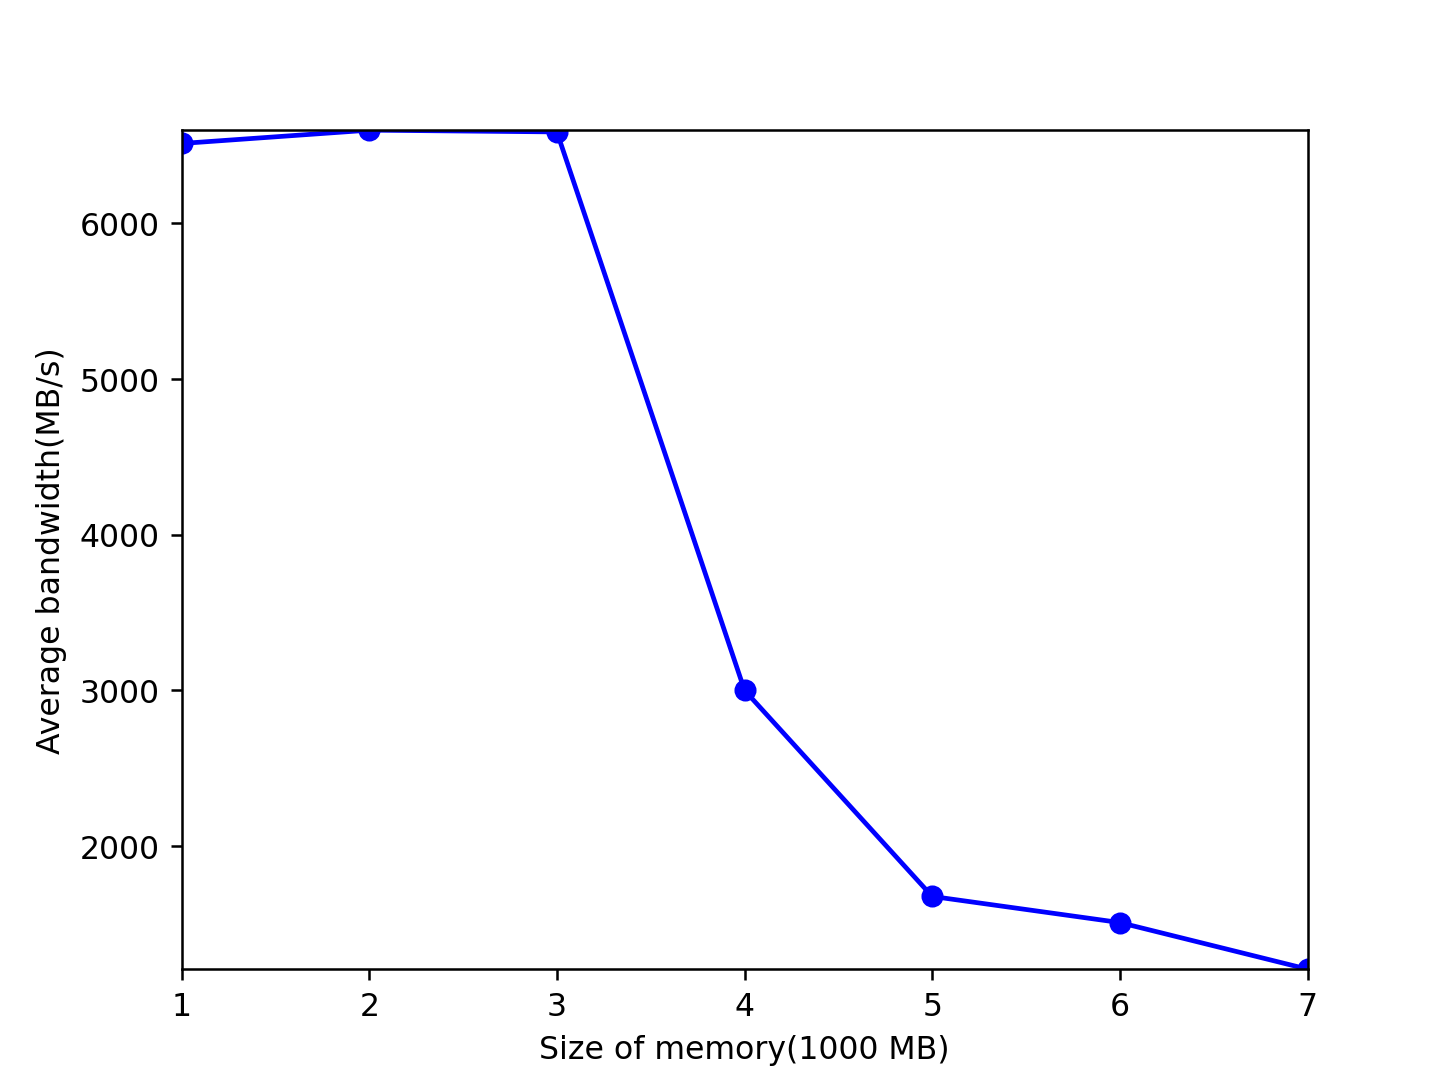
\includegraphics[width=7cm,height=7cm]{bandwidth.png} \label{X}}
    \hfill
    \subfloat[]{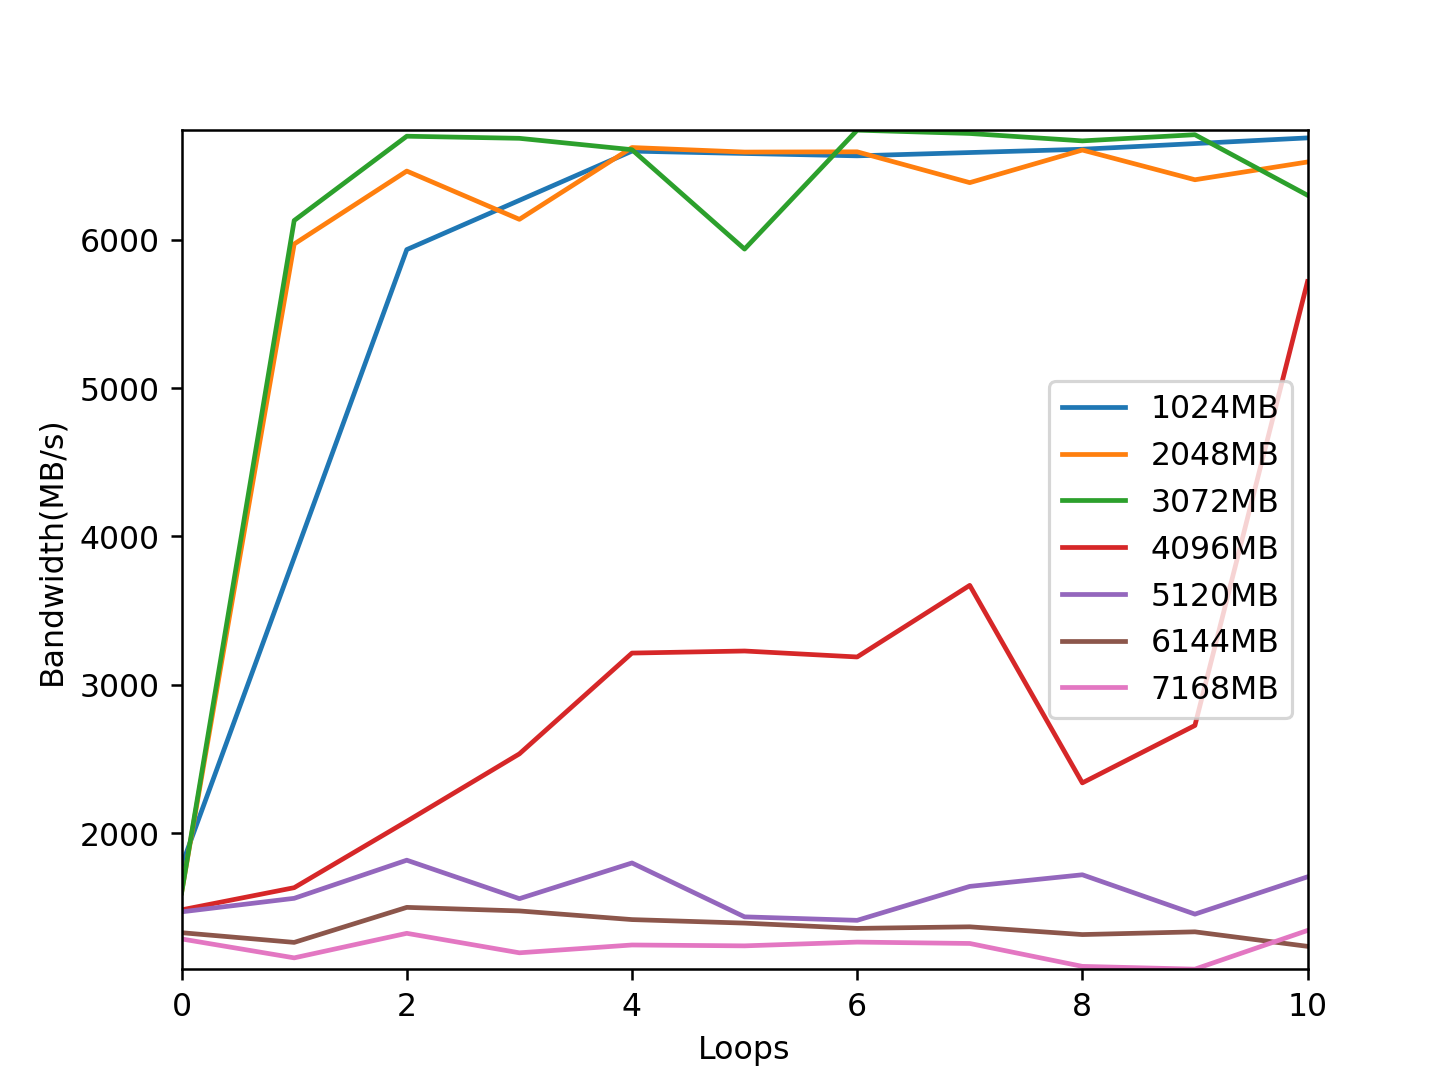
\includegraphics[width=7cm,height=7cm]{loops.png} \label{Y}}
	\caption{Question5}
\end{figure*}

\begin{large}
	\noindent Question6\\
\end{large}
\hspace*{2em}当尝试mem更大内存时,会发现进程被迫结束。这里经过几次尝试,发现差不多到总内存的20\%左右就会分配失败了。\\

\begin{LARGE}
    \noindent Chapter22\\
\end{LARGE}
\begin{large}
	\noindent Question1\\
\end{large}
\hspace*{2em}经过计算,可以得到在不同的随机种子和策略下的命中率如下:\\
\begin{tabular}{p{4cm}p{4cm}p{4cm}p{3cm}}  % 其中,tabular是表格内容的环境;c表示centering,即文本格式居中;c的个数代表列的个数
    \toprule[2pt]
    seed & policy & hit-rate & hit的项 \\ %中间用 & 隔开, 换行用\\
    \midrule[2pt]
    0    & FIFO       & 10\%    & 6          \\
    0    & LRU        & 20\%     & 6,9         \\
    0    & OPT  & 40\%   & 6,7,9,10           \\
    1    & FIFO   & 20\%           &  6,10   \\
    1    & LRU       & 20\%        &  6,10     \\
    1    & OPT       & 30\%        & 6,8,10      \\
    2    & FIFO   & 40\%           & 2,4,9,10  \\
    2    & LRU   & 40\%    & 2,4,9,10\\
    2    & OPT      & 40\%         & 2,4,9,10       \\
    \bottomrule[2pt]
\end{tabular}
\newpage
\begin{large}
	\noindent Question2\\
\end{large}
\hspace*{2em}通过以下三条指令:"python3 ./paging-policy.py --addresses=0,1,2,3,4,5,0,1,2,3,4,5 --policy=FIFO --cachesize=5 -c",
"python3 ./paging-policy.py --addresses=0,1,2,3,4,5,0,1,2,3,4,5 --policy=LRU --cachesize=5 -c",
"python3 ./paging-policy.py --addresses=0,1,2,3,4,5,4,5,4,5,4,5 --policy=MRU --cachesize=5 -c".就能得到最差的表现,此时的命中率都是0。为了提高效率,我们只需提高1的cache大小;此后命中率有很大提升,都提到了50\%。\\

\begin{large}
	\noindent Question3\\
\end{large}
\hspace*{2em}这里使用"python3 ./paging-policy.py -s 0 -n 10"指令,随机生成。再考虑使用不同的策略;根据不同的策略进行计算,以及通过-c标志验证,可以得到以下命中率:FIFO-10\%; LRU-20\%; OPT-40\%; UNOPT-0\%; RAND-0\%; CLOCK-0\%.\\

\begin{large}
	\noindent Question4\\
\end{large}
\hspace*{2em}这里随机生成32个数 10,9,9,11,7,6,6,7,6,3,4,6,6,5,5,6,6,2,2,1,2,3,3,1,1,2,0
,3,4,3,6,5,8;调用命令:"python3 ./paging-policy.py --addresses=10,9,9,11,7,6,6,7,6,3,4,6,6,5,5,6,6,2,
2,1,2,3,3,1,1,2,0,3,4,3,6,5,8 --policy=?"来计算。得到如下命中率:
LRU-48.48\%; RAND-42.42\%; CLOCK(bit-1)-36.36\%; CLOCK(bit-2)-39.39\%。\\

\begin{large}
	\noindent Question5\\
\end{large}
\hspace*{2em}首先这里我们要将生成的进行转化,主要用到了下面几行代码,根据掩码进行操作。之后就像前面一样,得结果,绘图分析。最终结果如下:
\begin{python}
for line in traceFile:
    if (not line.startswith('=')):
        vpnFile.write(str((int("0x" + line[3:11], 16) & 0xfffff000) >> 12) + "\n")
\end{python}
\begin{figure}[h]
    \centering
    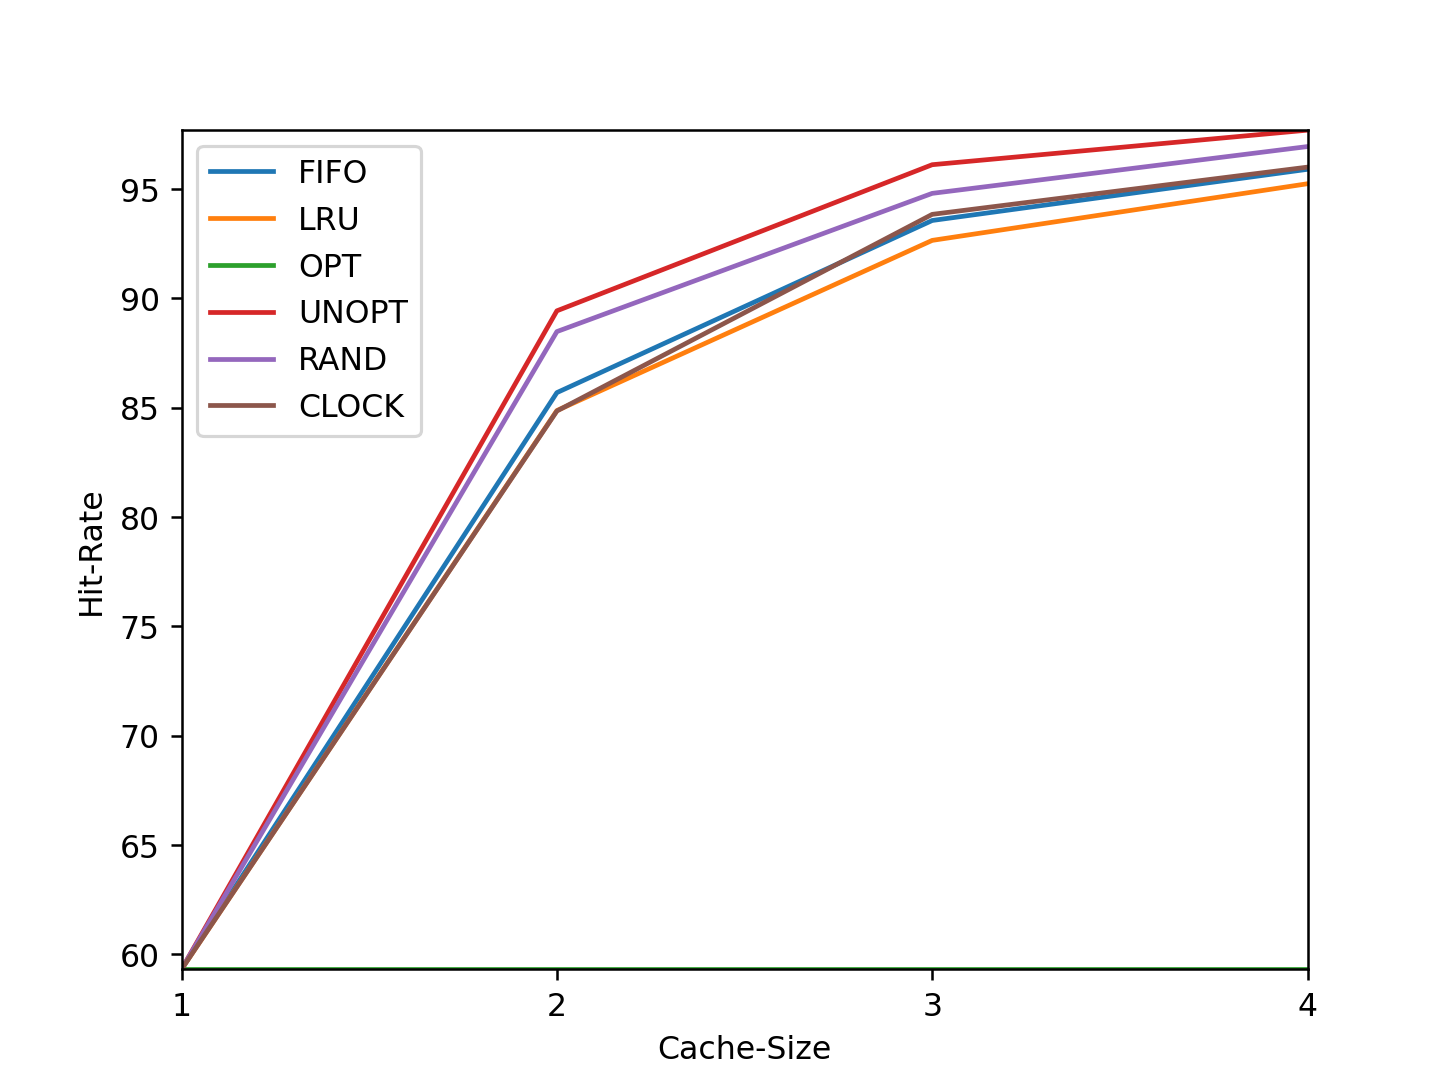
\includegraphics[width=8cm,height=6cm]{workload.png}
\end{figure}
\end{document}